\documentclass[12pt,a5paper]{memoir}
\usepackage{listings}
\usepackage{xcolor}
\usepackage{hyperref}
\usepackage{graphicx}


\lstset{
    backgroundcolor=\color{lightgray},
    basicstyle=\ttfamily,
    breaklines=true
}

\lstdefinelanguage{JavaScript}{
  morekeywords=[1]{break, continue, delete, else, for, function, if, in,
    new, return, this, typeof, var, void, while, with},
  % Literals, primitive types, and reference types.
  morekeywords=[2]{false, null, true, boolean, number, undefined,
    Array, Boolean, Date, Math, Number, String, Object},
  % Built-ins.
  morekeywords=[3]{eval, parseInt, parseFloat, escape, unescape},
  sensitive,
  morecomment=[s]{/*}{*/},
  morecomment=[l]//,
  morecomment=[s]{/**}{*/}, % JavaDoc style comments
  morestring=[b]',
  morestring=[b]"
}[keywords, comments, strings]

\title{A Smart Guide to Building Web Applications}
\author{João Costa Seco}
\begin{document}

\maketitle

\tableofcontents

\chapter{Introduction}

This small booklet has X parts illustrating small aspects of the construction of
a web server in JavaScript, a static web page using basic technologies like HTML
and CSS. And then how to develop a dynamic web page with events and dynamic
construction of HTML elements. 

The goal of this booklet is to illustrate the different aspects of the
construction of a web server in TypeScript. The booklet is not intended to be a
complete reference, but rather a quick guide to get you started.

\part{A Web Server in TypeScript}

\chapter{Setting up your first node application}

To start this adventure, we will start by setting up a simple \texttt{Node.js}
application. This will allow us to run JavaScript and TypeScript code outside of
the browser. Node.js is a JavaScript runtime environment that allows us to run
JavaScript and TypeScript code outside of the browser.

\begin{enumerate}

\item 
To start with you need to install \texttt{Node.js} in your computer. You can download it from the
\href{https://nodejs.org}{Node.js} website.
%
Next, we are going to use command line instructions and a text editor. The
recommended editor for this journey is Visual Studio Code, with a few plug-ins
that will be highlighted along the way. 

\item To start, you need to create a directory for your project and initialize
it.

\begin{lstlisting}[language=bash]
mkdir myproject
cd myproject
npm init -y
\end{lstlisting}

These commands will add a \texttt{package.json} file to your project. This file
contains all the configuration information for your project.

\item Next, you need to install the TypeScript compiler and initialize it.

\begin{lstlisting}[language=bash]
npm install -g typescript
tsc --init
npm install ts-node typescript --save-dev
\end{lstlisting}

These commands will add the file \texttt{tsconfig.json} to your project and
install the necessary packages. This will contain the information for the
TypeScript compiler to compile your code.

\item Next, you need to write your first TypeScript file. Create a file called
\texttt{index.ts} in a folder called \texttt{src}.

\begin{lstlisting}
console.log("Hello World");
\end{lstlisting}

\item Change your \texttt{package.json} file and modify the "start" script to run your program.

\begin{lstlisting}[language=JavaScript]
"scripts": {
    "start": "ts-node src/index.ts"
},
\end{lstlisting}

\item Finally, you can run your program with the following command:

\begin{lstlisting}[language=bash]
npm start
\end{lstlisting}

You should see the message "Hello World" printed in the console.
Congratulations, you have succeeded in writing and running your first TypeScript
application.

\end{enumerate}

\chapter{Setting up your first web server}

A Web server is a program that listens to requests from a browser and returns a
response. Responses can be HTML pages, images, JSON data, etc. Content can be
either static if provided by an existing file in the server filesystem, or
dynamic if it is created on demand and based on the information from the request.

\begin{enumerate}

\item Start by clearing the \texttt{index.ts} file. To start designing a basic
web server, we will use the \texttt{http} module. Write the following declarations into the 
\texttt{index.ts} file.

\begin{lstlisting}
  import http from 'http'
\end{lstlisting}

\item Then we need some constants to determine the address and port of our
server. Write the following declarations next to the previous one.

\begin{lstlisting}
const host = 'localhost';
const port = 8080;
\end{lstlisting}

\item Next, we need to write a function that will handle the requests. This
function accepts two objects as parameters: the request and the response. For
now, we are just going to return a simple HTML page for all requests. Write the
following code in the \texttt{index.ts} file.

\begin{lstlisting}
function doRequests(
    req:IncomingMessage, 
    res:ServerResponse) {

  const page = `
    <HTML>
      <BODY>
        Hello, World! from the server
      </BODY>
    </HTML>
  `
  res.setHeader("Content-Type", 
                "text/html");
  res.writeHead(200)
  res.end(page)
}
\end{lstlisting}
  
Notice that the immutable variable \texttt{page} contains the HTML code for a
simple page and that the object \texttt{res} is used to set the headers, and the
return code of the response. The \texttt{end} method is used to send the result
to the browser, in the body section. Notice the use of the backtick quotes to
define a string over several lines in the file.

Since we need to use type annotations for the function parameters, we need to
import types \texttt{IncomingMessage} and \texttt{ServerResponse}. So, we need to update
our import statement to include these.

\begin{lstlisting}
  import http, {IncomingMessage, ServerResponse} from 'http'
\end{lstlisting}

\item Next, we need to create the server and start listening to requests. Write
the following code in your file:

\begin{lstlisting}
const server = 
  http
  .createServer(doRequests);

server.listen(
  port, 
  host, 
  () => {
    console.log(`Server is running on http://${host}:${port}`);
  }
);
\end{lstlisting}

We first create an object called \texttt{server} based on the previously defined
function doRequests. Then we call the \texttt{listen} method on the server
object to start listening to requests. The \texttt{listen} method accepts three
parameters: the port, the host, and a callback function that is called when the
server is ready to accept requests.
%
In this case, the backtick quotes are used to define an interpolated string with
the host and port values.

\item
Your \texttt{index.ts} file should look like this by now:

\begin{lstlisting}
import http, {IncomingMessage, ServerResponse} from 'http'
const host = 'localhost';
const port = 8080;

function doRequests(
  req:IncomingMessage, 
  res:ServerResponse) {
    const page = `
        <HTML>
          <BODY>
            Hello, World! from the server
          </BODY>
        </HTML>
        `
    res.setHeader("Content-Type", "text/html");
    res.writeHead(200)
    res.end(page)
}

const server = 
  http
  .createServer(doRequests);

server.listen(
  port, 
  host, 
  () => {
    console.log(`Server is running on http://${host}:${port}`);
  }
);
\end{lstlisting}


\item Finally, you can run your program with the following command:


\begin{lstlisting}[language=bash]
npm start
\end{lstlisting}
  
You should see the message "Server is running on http://localhost:8080" printed
  in the console. If you go to a browser and use that same URL, you should see 
  
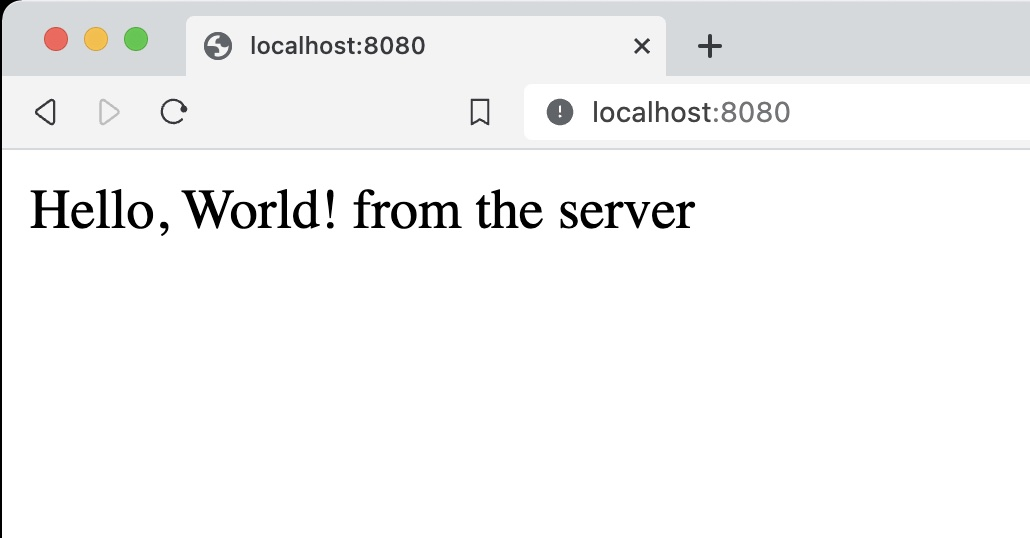
\includegraphics[width=\linewidth]{WebServer1.jpg}
  
  Congratulations, you have succeeded in writing and running
  your webserver using TypeScript.

  (You can find the final code in the file \texttt{index.ts} in the folder
  chapter2 of this guide.)

\end{enumerate}

\chapter{Returning a 404 error}

\begin{lstlisting}
a
\end{lstlisting}

\chapter{Loading files from the web server}

\begin{lstlisting}

\end{lstlisting}


  


\chapter{Returning dynamic content}

Use a form to upload parameters.

\chapter{Webservices: returning JSON data}

\part{A Web page using HTML and CSS}

\chapter{HTML: Writing your first web page}

\chapter{HTML: The anatomy of an HTML element}

\chapter{HTML: Basic Text Formatting}

\chapter{HTML: Adding images}

\chapter{HTML: Linking different pages}

\chapter{HTML: Formatting with stylesheets}

\chapter{HTML: Basic Layout with CSS}

\chapter{HTML: Making requests with Forms}

\part{Reactive pages: Events and JavaScript}

\part{Dynamic pages with JavaScript}

\end{document}